\documentclass[a4paper,10pt]{article}
\usepackage[utf8]{inputenc}
\usepackage[UKenglish]{babel}
\usepackage{fancyhdr}
\usepackage{anysize}
\usepackage{amsmath,amssymb,amsfonts,amsthm} % Typical maths resource packages
\usepackage{lastpage}
\usepackage[all]{xy}  % drawings
%\usepackage{listings} % code highlighting
\usepackage[usenames,dvipsnames]{color}
\usepackage{graphicx}
\usepackage{caption}
\usepackage{subfigure}
\usepackage{upgreek}

\pagestyle{fancy}
\fancyfoot[R]{\em \thepage / \pageref{LastPage}}
\fancyfoot[C]{}
\fancyfoot[L]{\em Master VIBOT}
\fancyhead[R]{\em Lab4 - EKF Map Based Localization}
\fancyhead[C]{}
\fancyhead[L]{\em Probabilistic Robotics}
\renewcommand{\headrulewidth}{0.4pt}
\renewcommand{\footrulewidth}{0.4pt}

%\,	 a small space
%\:	 a medium space
%\;	 a large space
%\quad	 a really large space
%\qquad	 a huge space
%\!	 a negative space (moves things back to the left)
        
\begin{document}

\marginsize{2cm}{2cm}{2cm}{2cm}

% Title
%\hspace{1mm}
\begin{center}
\Large \textbf{Lab4 - EKF Map Based Localization}
\end{center}
%\hspace{1mm}

\section{Introduction}

The goal of this Lab exercise is to program an EKF Map Based Localization algorithm to work with data taken from a real Turtlebot.

Map based localization is a concept that in real life each one of us uses whenever we go to a new place. When a human being goes to a new environment it tries to know where he is. In order to do that, what he does is to read a map of the place and try to relate key parts of the environment he has seen with features of the map so he can localize himself in the map while he is moving around. This can be applied also to robots using an EKF map based localization algorithm:

\begin{center}
	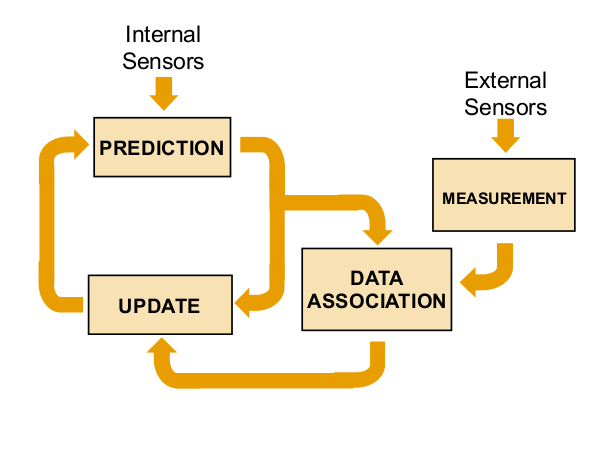
\includegraphics[width=0.35\textwidth]{pict/ekf_pic.png}
	\captionof{figure}{Schematic of EKF map based localization}
	\label{measur}
\end{center}

The EKF map based localization is based on two different steps, prediction and update. The prediction is based on the internal odometry of the Turtlebot, while the update is based on lines sensed by its Kinect RGB-D sensor.

\section{Pre-lab}

Read and understand all the guide for this Lab and look about the EKF algorithm in your lecture slides. The pre-lab consists in finding the equations for the update step, where you need to transform world referenced lines $(\rho_w, \varphi_w)$ of the known map to robot referenced lines $(\rho_r, \varphi_r)$ (look at Fig.~\ref{ex}).

Define the expected measurement equations $h(x_{k|k-1})$ and calculate the jacobian $H$ of the expected measurement with respect to the robot state $x_{k|k-1}$.
\begin{center}
	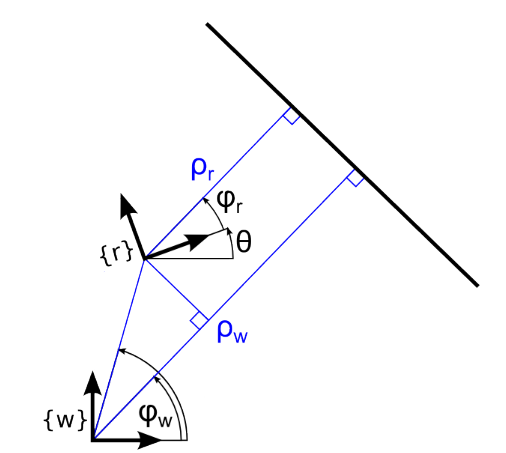
\includegraphics[width=0.40\textwidth]{pict/find_h.png}
	\captionof{figure}{Schematic to deduce the measurement function $h(x_{k|k-1})$}
	\label{ex}
\end{center}

You can write them in paper and attach a picture in the online form submission.

\section{Lab work}

The ROS package named \texttt{lab4\_ekf} contains the skeleton code for running this lab. The input messages are odometries from the turtlebot (\texttt{nav\_msgs/Odometry}) and lines coming from the Split and Merge algorithm (\texttt{visualization\_msgs/Marker}). You can test the code by running:
\begin{verbatim}
    roslaunch lab4_ekf ekf.launch
\end{verbatim}
\noindent
As you can see in Rviz that the robot doesn't move at all. The original data from the robot can be seen in red and the filtered one in blue. You will need to complete the code inside the \texttt{ekf\_localization.py} file in order to complete properly the EKF Localization algorithm. No changes are needed in the \texttt{node.py}. Remember that you have useful functions in the library \texttt{functions.py}. If you think you need to modify any of these files ask your lab assistant first. The EKF algorithm goes as follows:
\begin{align*} \scriptsize
    & \blacktriangleright \textit{\textbf{Pose initialization}}\\
    & x_0 = \hat{x}_0 \\
    & P_0 = \hat{P}_0 \\
    & \textbf{for } \text{k} = 1 \textbf{ to } steps \textbf{ do:} \\
    & \qquad \left[ u_k^{R_{k-1}}, Q_k \right] = get\_odometry() \\
    & \qquad \blacktriangleright \textit{\textbf{EKF prediction}}\\
    & \qquad \left[ x_{k|k-1}, P_{k|k-1} \right] = move\_vehicle(x_{k-1}, P_{k-1}, u_k, Q_k) \\
    & \qquad \left[ z_k, R_k \right] = get\_measurements() \\
    & \qquad \blacktriangleright \textit{\textbf{Data association}}\\
    & \qquad \mathcal{H}_k = data\_association(x_{k|k-1}, P_{k|k-1}, z_k, R_k) \\
    & \qquad \blacktriangleright \textit{\textbf{EKF update}}\\
    & \qquad \left[ x_k, P_k \right] = update\_position(x_{k|k-1}, P_{k|k-1}, z_k, R_k) \\
    & \textbf{end for}
\end{align*}

\subsection{EKF prediction}

You will need to complete the function \texttt{predict} inside \texttt{ekf\_localization.py}. This part of the algorithm is where, from the odometry $\vec{u}_k$ and the previous position the new one is computed. 
\begin{align*}
    & \blacktriangleright \textit{\textbf{Prediction}}\\
    & x_{k|k-1} = f(x_{k-1} ,u_k, w_k) \\
    & P_{k|k-1} = A_k P_{k-1} A_k^T + W_k Q_k W_k^T
\end{align*}
These measurements have an uncertainty associated. This uncertainty has been estimated to be 0.025 m as linear noise and 2 degrees as angular noise, so the $Q_k$ matrix can be estimated for all the measurements as:
\begin{align}
    \label{q_k}
    Q_k &= \begin{pmatrix}
	    0.025 & 0 & 0\\0 & 0.025 & 0\\ 0 & 0 & \textnormal{deg2rad}(2)
	\end{pmatrix}
\end{align}

\begin{center}
	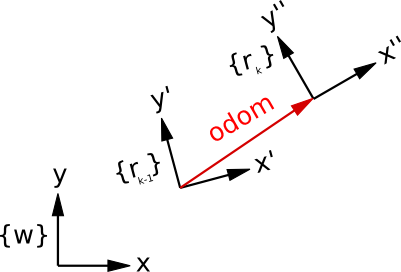
\includegraphics[width=0.30\textwidth]{pict/prediction.png}
	\captionof{figure}{Schematic of the odometry measurement. Remember that robot position is defined in the world frame (W) while odometry is measured in the robot frame (R).}
	\label{odometry}
\end{center}

Once implemented correctly, when you test the script you should see the robot (blue arrow) moving around the room, and an ellipse representing uncertainty increasing its size when the robot moves.

\begin{center}
	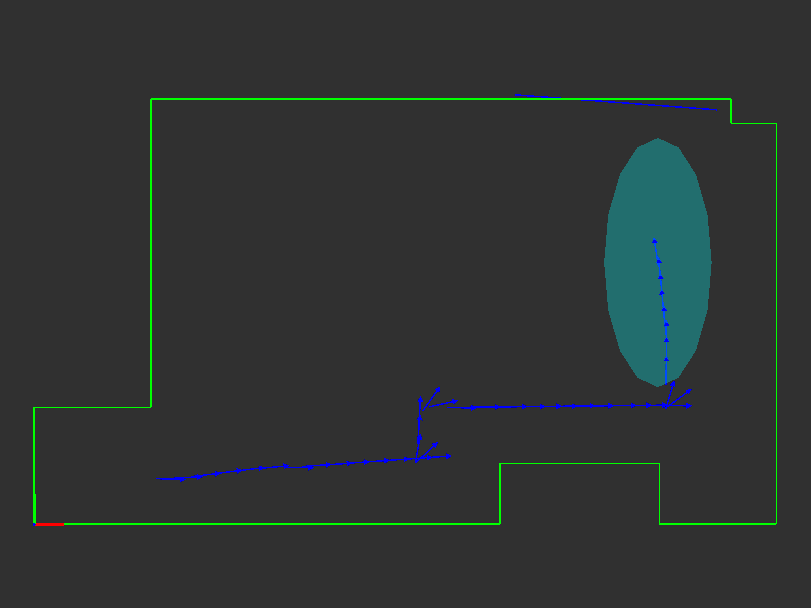
\includegraphics[width=0.40\textwidth]{pict/uncert.png}
	\captionof{figure}{Prediction without updates.}
	\label{no_updates}
\end{center}


\subsection{Data association}

Data association is the main parts in the algorithm. It tries to match the line measurements with the a priori known map of the environment. If data association is carried correctly the filter updates will be meaninfull and the robot will be correctly located.

To decide whether or not the distance between a feature and an observation is close enough both uncertainties have to be taken into account. Mahalanobis distance must be used.

Each measured line is compared to all lines in the known map. The smallest Mahalanobis distance is kept. If this distance is smaller than chi-square $\upchi_{\rho,\varphi}^2$ test threshold, the line is considered associated and can be used in the update. You can choose this parameter.
\begin{align*}
    & \blacktriangleright \textit{\textbf{Data association}}\\
    & v_{ij} = z_i - h(x_{k|k-1}) \\
    & S_{ij} = H_j P_{k|k-1} H_j^T + R_i \\
    & D_{ij}^2 = v_{ij}^T S_{ij}^{-1} v_{ij} \\
    & \text{Take the smallest } D_{ij}^2 \text{ if } D_{ij}^2 < \upchi_{\rho,\varphi}^2
\end{align*}

To obtain the expected measurement function $h(x_{k|k-1})$ that transforms a feature from the real map in polar coordinates in the world frame ${}^Wx_f$ to a feature in polar coordinates in the robot frame ${}^Rx_f$ you can use  Fig.~\ref{measur} for guidance.
\begin{center}
	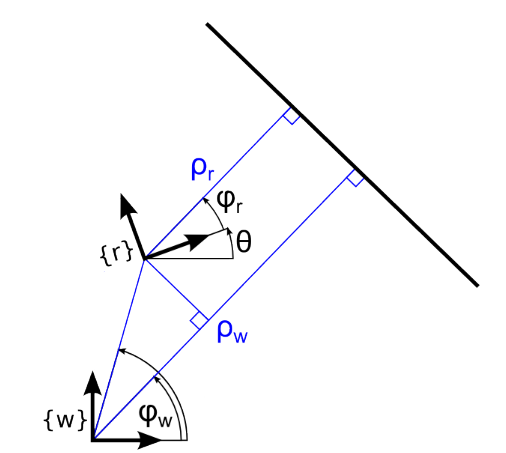
\includegraphics[width=0.30\textwidth]{pict/find_h.png}
	\captionof{figure}{Schematic to deduce the measurement function $h(x_{k|k-1})$}
	\label{measur}
\end{center}

Regarding $R_k$, the covariance matrix for the observations, the angle measurement noise has been estimated to 10 degrees and the range measurement to 0.2 m. $R_k$ matrix is estimated as constant.
\begin{align}
    \label{R_k}
    R_k &= \begin{pmatrix}
        0.2 & 0 \\
        0 & \textnormal{deg2rad}(10)
    \end{pmatrix}
\end{align}

\subsection{Update}

In this step, the matches obtained on the data association are used to update the position of the robot and its uncertainty. The main algorithm is the following one. Starting by calculating the innovation $v_k$ which is the difference between the observed features $z_k$ and the expected observation $h(x_{k|k-1})$. Then the uncertainty of this innovation is calculated in $S_k$. Finally. the Kalman gain $K_k$ is computed allowing to update the state vector $x_k$ and the covariance matrix $P_k$.
\begin{align*}
    & \blacktriangleright \textit{\textbf{Update}}\\
    & v_k = z_k - h(x_{k|k-1}) \\
    & S_k = H_k P_{k|k-1} H_k^T + R_k \\
    & K_k = P_{k|k-1}  H_k^T S_k^{-1} \\
    & x_k = x_{k|k-1} + K_k v_k \\      
    & P_k = \left( I - K_k H_{k} \right) P_{k|k-1} \left( I - K_k H_{k} \right)^T + K_k R_k K_k^T
\end{align*}

Note that $h(x_{k|k-1})$ and $H_k$ have already been computed for each feature in the data association. In this step the difference is that both can have more than one observation to update the robot position. In order to update with all the information at the same time $h(x_{k|k-1})$ and $H_j$ computed for each observation associated to a feature are stacked vertically to obtain the final $h(x_{k|k-1})$ and $H_k$ matrix and be able to run the update algorithm.

\begin{center}
	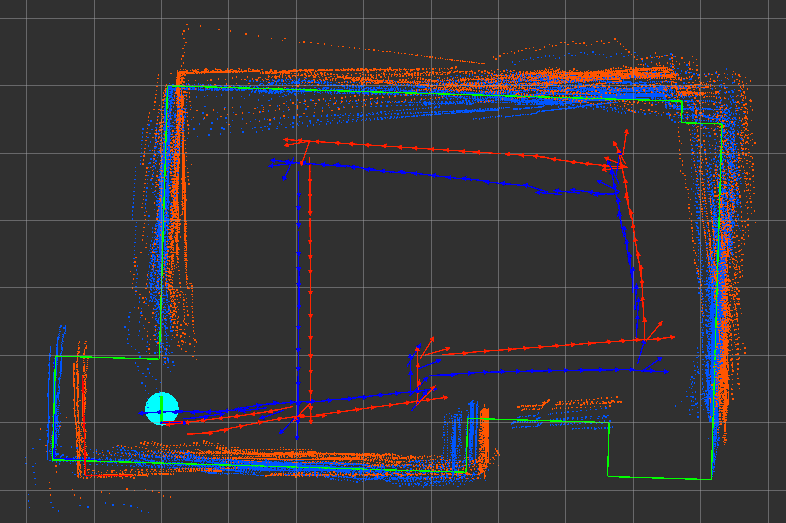
\includegraphics[width=0.40\textwidth]{pict/lab4_comp.png}
	\captionof{figure}{Comparison between raw data (red) with EKF (blue). Known map in green.}
	\label{updates}
\end{center}

\section{Optional}

Using polar representation introduces a new challenge. Walls are represented by lines without ends and not by segments. These can introduce confusions in the data association. Try adding new constraints in the data association subsection to avoid matching the sensed lines with "ghost" walls.

\section{Lab report}

Write a brief report in less than 4 pages explaining your solution and problems faced. Include the final code and the report in a zip file.

\end{document}
